\documentclass{beamer}
\usetheme{Madrid}

\usepackage[utf8]{inputenc}
%\usepackage{beamerthemeshadow}
%\usepackage{stmaryrd} % Needed for \bigsqcap
%\usepackage{algorithm}
%\usepackage{algpseudocode}


\definecolor{Green}{rgb}{0.506, 0.727, 0.396} % (primary)

\usecolortheme[named=Green]{structure}

\newcommand\owlIndent{\hspace{4mm}}
\newcommand\setspacing{\hspace{2pt}}

\renewcommand{\arraystretch}{1.2} % Vertical spacing of rows in table



\begin{document}
\title{Existential restrictions}
\author{Henriette Harmse}
\date{}

\frame{\titlepage}
%\AtBeginSection[]
%{
%  \begin{frame}<beamer>
%    \frametitle{Outline}
%    \tableofcontents[]
%  \end{frame}
%}


\frame{\frametitle{Prerequisites}
	Before doing this tutorial you need to have the following knowledge:	
	\begin{enumerate}
		\item Building blocks of OWL and Description Logics.
		\item \texttt{SubClassOf} vs \texttt{EquivalentTo}
	\end{enumerate}
}

\frame{\frametitle{Qualified existential restrictions}
	\begin{block}{Syntax}
	\begin{table} 
		\begin{center} 
			\begin{small}
				\begin{tabular}{|c|c|} 
					\hline					
					\textbf{OWL}&\textbf{DL}\\
					\hline 
					\begin{minipage}{5cm}
						$\begin{aligned}
							&\texttt{ObjectProperty: r}\\
							&\texttt{Class: D}\\
							&\owlIndent\texttt{EquivalentTo: r some C}\\
							&\texttt{Class: C}
						\end{aligned}$
					\end{minipage}				
					& 
					\begin{minipage}{2cm}
						$\begin{aligned}
							D \equiv \exists r.C
						\end{aligned}$
					\end{minipage}										
					\\
					\hline						 				  
				\end{tabular}
			\end{small}
		\end{center}
	\end{table}
\end{block}
\begin{block}{Semantics}
	\begin{itemize}
		\item $(\exists r.C)^{\mathcal{I}} = \{x \in \triangle^{\mathcal{I}} | \text{there is an } y \in \triangle^{\mathcal{I}} \text{ such that } (x, y) \in r^{\mathcal{I}} \text{ and } y \in C^{\mathcal{I}}\}$
		\item \texttt{r some C} ($\exists r.C$) is the set of individuals such that for each individual $x$ there is at least 1 individual $y$ of type $C$ that is linked to $x$ via the object property (role) $r$.
	\end{itemize}
\end{block}
}


\frame{\frametitle{Qualified existential restrictions}
	\begin{block}{Example using \texttt{EquivalentTo}}
		$\begin{aligned}
			&\texttt{ObjectProperty: owns}\\
			&\texttt{Class: PetOwner}\\
			&\owlIndent\texttt{EquivalentTo: owns some Pet}\\
			&\texttt{Class: Pet}
		\end{aligned}$
	\end{block}	
	\begin{block}{Example using \texttt{SubClassOf}}
		$\begin{aligned}
			&\texttt{ObjectProperty: owns}\\
			&\texttt{Class: DogOwner}\\
			&\owlIndent\texttt{SubClassOf: owns some Pet}\\
			&\texttt{Class: Pet}
		\end{aligned}$
	\end{block}		
 
}

\frame{\frametitle{Qualified existential restrictions}
\begin{block}{Examples}
	Which of these individuals will be in \texttt{r some C} and therefore as well in \texttt{D}?\\
	\medskip
	\includegraphics[trim = 0mm 0mm 0mm 0mm, clip, scale=0.3]{./images/QualifiedRestrictionExamples.png}
\end{block}	
	
	
	%trim option's parameter order: left bottom right top
%	\includegraphics[trim = 63mm 0mm 0mm 20mm, clip, scale=1]{QualifiedRestrictionExamples.png} 
}


\frame{\frametitle{Qualified existential restrictions}
	\begin{block}{Examples}
		Which of these individuals will be in \texttt{r some C} and therefore as well in \texttt{D}?\\
		\medskip
		\includegraphics[trim = 0mm 0mm 0mm 0mm, clip, scale=0.3]{./images/QualifiedRestrictionExamples.png}
	\end{block}	
	
	\begin{block}{Answer}
		Individuals 2, 3, 5	
	\end{block}
}


\frame{\frametitle{Variations on existential restrictions}
	\begin{block}{Syntax}
		\begin{table} 
			\begin{center} 
				\begin{small}
					\begin{tabular}{|c|c|c|} 
						\hline					
						\textbf{Name}&\textbf{OWL}&\textbf{DL}\\
						\hline
						\begin{minipage}{1.5cm}
						Unqualified existential restrictions
					    \end{minipage}
						& 
						\begin{minipage}{5cm}
							$\begin{aligned}
								&\texttt{ObjectProperty: owns}\\
								&\texttt{Class: Owner}\\
								&\owlIndent\texttt{EquivalentTo:} \\
								&\owlIndent\owlIndent\texttt{owns some owl:Thing}
							\end{aligned}$
						\end{minipage}	
						& 
						\begin{minipage}{4cm}
							$\begin{aligned}
								Owner \equiv \exists owns \top
							\end{aligned}$
						or\\
							$\begin{aligned}
								Owner \equiv \exists owns
							\end{aligned}$						
						\end{minipage}																		
						\\
						\hline	
						\begin{minipage}{1.5cm}
						Value restrictions
						\end{minipage}
						& 
						\begin{minipage}{5cm}
							$\begin{aligned}
								&\texttt{ObjectProperty: citizenOf}\\
								%&\owlIndent\owlIndent\texttt{citizenOf}\\
								&\texttt{Class: UKCitizen}\\
								&\owlIndent\texttt{EquivalentTo:} \\
								&\owlIndent\owlIndent\texttt{citizenOf hasValue UK} \\
								&\texttt{Individual: UK}
							\end{aligned}$
						\end{minipage}	
						& 
						\begin{minipage}{4cm}
							$\begin{aligned}
								UKCitizen &\equiv\\
								 &\exists citizenOf.\{UK\}
							\end{aligned}$				
						\end{minipage}																		
						\\
						\hline	
						\begin{minipage}{1.5cm}
							Existential restriction on data property
						\end{minipage}
						& 
						\begin{minipage}{5cm}
							$\begin{aligned}
								&\texttt{DataProperty: name}\\
							%	&\owlIndent\owlIndent\texttt{name}\\
								&\texttt{Class: Human}\\
								&\owlIndent\texttt{SubClassOf:} \\
								&\owlIndent\owlIndent\texttt{some name xsd:string}
							\end{aligned}$
						\end{minipage}	
						& 
						\begin{minipage}{4cm}
							$\begin{aligned}
								Human &\sqsubseteq \\
								& \exists name.\texttt{xsd:string} 
							\end{aligned}$				
						\end{minipage}																		
						\\
						\hline															 				  
					\end{tabular}
				\end{small}
			\end{center}
		\end{table}
	\end{block}
}

\end{document}
